\begin{frameExample}{Dieta}{}
  % EXAMPLE 2.6-2 {Diet Problem} Gupta
  La persona quiere decidir los componentes de una dieta que cumpla con sus requerimientos diarios de proteínas, grasas y carbohidratos al costo mínimo. La elección debe hacerse a partir de cuatro tipos diferentes de alimentos. Los rendimientos por unidad de estos alimentos se dan en la tabla siguiente. Formule un modelo de programación lineal para el problema.
  
  {\centering
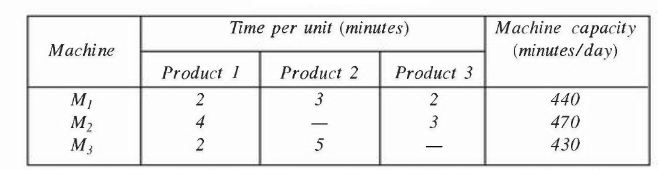
\includegraphics[scale=0.5]{example_allocation_gupta}
\par}

  
\end{frameExample}



%%% Local Variables:
%%% mode: latex
%%% TeX-master: "../slides"
%%% End:
